We only sketch \MMT here to the extent that we need it and refer to \cite{RabKoh:WSMSML13} for details.
An OMDoc/MMT theory graph is a diagram in the category of \MMT theories and theory morphisms.
Theories represent all kinds of languages such as mathematical foundations and type systems as well as individual mathematical theories.
Theory morphisms represent relations between them including translations, imports, and representation theorems.

\paragraph{Theories}
In the simplest case an \MMT \textbf{theory} is a finite list of symbol declarations.
Each \textbf{symbol declaration} must have a name and may optionally have a type object, a defining object, and arbitrary meta-data (such as tags, cross-references, comments, etc).
The \textbf{objects} are OpenMath 2.0 objects \cite{BusCapCar:2oms04} --- these are complex expressions formed from application, binding, variables, literals, and symbol references.

Critically, \MMT enforces structural validity: Every object may only reference symbols that are declared in or imported into the containing theory.
But \MMT abstracts from the foundational semantics such as type and logic systems that specify exactly which objects are meaningful.
This puts \MMT into a powerful intermediate position, where enough structure is guaranteed for knowledge management while not committing to a particular foundation.

An example MMT theory can be found in Listing~\ref{lst:mmt-odk-int}.
The theory \texttt{Int} shows a part of the formalisation of integers including comments.
Here the namespace is just a URI that is used to form globally unique URIs for all subsequent knowledge items.
As described above, each symbol declaration may consist of multiple components: types are prefixed with \texttt{:}, definitions with \texttt{=}, and notations with \texttt{\#}.

\lstinputlisting[language=MMT,mathescape,basicstyle=\footnotesize\sf,
  caption={Example of an MMT theory: Defining a theory of integers. },
  label=lst:mmt-odk-int
]{examples/odk-int.mmt}

Above we have skipped the \MMT module system, which is not essential for our results here.
In the simplest case, include declarations import declarations from other theories. Above this is used to include the theory \cn{Logic} into the theory \cn{Int}. (The $?$ character occurs to form the URI of a theory relative to the current namespace.)
Moreover, there is one detail of the \MMT module system that is critical for \pn: Every theory may have a \textbf{meta-theory}.
Above, the meta-theory of \cn{Int} is \cn{LF}.
Practically, the meta-theory mostly behaves like an include.
But conceptually, the meta-theory of a theory $T$ is the language that provides the foundational background to understand $T$.
The most common use case employs three meta-levels: Firstly, an \MMT theory introduces a logical framework $F$.
Secondly, $F$ serves as the meta-theory of a foundation $L$, which uses the symbols of $F$ to define a particular type system and logic.
Thirdly, a library of mathematical knowledge is developed as a theory graph in which all theories have meta-theory $L$.

A sample theory graph can be found in Figure~\ref{fig:odk_theories}.
It contains some of the theories we make use of in our approach.

\begin{figure}[ht]\centering
  \providecommand\myxscale{3}
  \providecommand\myyscale{1.5}
  \providecommand\myfontsize{\footnotesize}
  \documentclass{standalone}
\usepackage{tikz}
\usetikzlibrary{backgrounds,shapes,fit,shadows,arrows,shapes.geometric}
\makeatletter%%%%%%%%%%%%%%%%%%%%%%%%%%%%%%%%%%%%%%%%%%%%%%%%%%%%%%%%%%%%%%%%%
% A TIKZ library for MMT Theory Graphs
% copyright 2014 Michael Kohlhase; Released under the LPPL
%%%%%%%%%%%%%%%%%%%%%%%%%%%%%%%%%%%%%%%%%%%%%%%%%%%%%%%%%%%%%%%%%
%
% this library provides some standardized node and arrow styles for formatting MMT graph
% diagrams in tikz. The advantage is that we can classify the arrows and nodes
% symbolically and with the styles in this library achieve a uniform look that helps
% readability. 
%
%%%%%%%%%%%%%%%%%%%%%%%%%%%%%%%%%%%%%%%%%%%%%%%%%%%%%%%%%%%%%%%%%

%%% 1. Theories
% a generic theory
\def\outerthysep{.3mm}
\def\innerthysep{.5mm}
\tikzstyle{thy}=[draw,outer sep=\outerthysep,rounded corners,inner sep=\innerthysep]
% a primitive theory
\tikzstyle{primthy}=[thy,double]
% a theory graph 
\tikzstyle{thygraph}=[draw,outer sep=1mm,rounded corners,dashed]

%%% 2. Arrows 
%%% 2.1. Arrowtips (only internal)
\usetikzlibrary{arrows}
\newcommand{\@mmtarrowtip}{angle 45}
\newcommand{\@mmtreversearrowtip}{angle 45 reversed}
\newcommand{\@mmtarrowtipepi}{triangle 45}
\newcommand{\@mmtarrowtipmonoright}{right hook}
\newcommand{\@mmtarrowtipmonoleft}{left hook}
\newcommand{\@mmtarrowtippartial}{right to}
\newcommand{\@mmtarrowtippartialleft}{left to}
\newcommand{\@mmtreversearrowtippartial}{right to reversed}
\newcommand{\@mmtreversearrowtippartialleft}{left to reversed}

%%% 2.2 the arrow sstyles in graphs
\usetikzlibrary{decorations,decorations.pathmorphing,decorations.markings}
% any morphism 
\tikzstyle{morph}=[-\@mmtarrowtip,thick] 
\tikzstyle{mapsto}=[|-\@mmtarrowtip] %| any morphism 
% structures
\tikzstyle{struct}=[-\@mmtarrowtip,thick]
% inclusions: regular, partial, and left variants
\tikzstyle{include}=[\@mmtarrowtipmonoright-\@mmtarrowtip,thick]
\tikzstyle{revinclude}=[\@mmtarrowtip-\@mmtarrowtipmonoright,thick]
\tikzstyle{pinclude}=[\@mmtarrowtipmonoright-\@mmtarrowtippartial,thick]
\tikzstyle{includeleft}=[\@mmtarrowtipmonoleft-\@mmtarrowtip,thick]
\tikzstyle{pincludeleft}=[\@mmtarrowtipmonoleft-\@mmtarrowtippartialleft,thick]
% views: regular, mono, partial, and left variants
\tikzstyle{preview}=[decorate,
                                decoration={coil,aspect=0,amplitude=1pt,
                                                    segment length=6pt,
                                                    pre=lineto,pre length=3pt,
                                                    post=lineto,post length=5pt},
                                thick]
\tikzstyle{view}=[preview,-\@mmtarrowtip]
\tikzstyle{mview}=[preview,\@mmtarrowtipmonoright-\@mmtarrowtip]
\tikzstyle{pview}=[preview,-\@mmtarrowtippartial]
\tikzstyle{pmview}=[preview,\@mmtarrowtipmonoright-\@mmtarrowtippartial]
\tikzstyle{viewleft}=[preview,-\@mmtarrowtip]
\tikzstyle{mviewleft}=[preview,\@mmtarrowtipmonoleft-\@mmtarrowtip]
\tikzstyle{pviewleft}=[preview,-\@mmtarrowtippartialleft]
\tikzstyle{pmviewleft}=[preview,\@mmtarrowtipmonoleft-\@mmtarrowtippartialleft]
\tikzstyle{adoption}=[preview,thin,double,-\@mmtarrowtip]
% biviews: regular, partial, and left variants
\tikzstyle{biview}=[preview,\@mmtarrowtip-\@mmtarrowtip]
\tikzstyle{pbiview}=[preview,\@mmtreversearrowtippartial-\@mmtarrowtippartial]
\tikzstyle{pbiviewleft}=[preview,\@mmtreversearrowtippartialleft-\@mmtarrowtippartialleft]
% defining views (experimental)
\tikzstyle{defview}=[preview,densely dotted,-\@mmtarrowtip]
% meta-theory inclusion
\tikzstyle{meta}=[dotted,-\@mmtarrowtip,thick]
% conservative extensions (abbreviation)
\tikzstyle{conservative}=[hooks-\@mmtarrowtip,double] 
% conservative development
\tikzstyle{conservdev}=[hooks-\@mmtarrowtip,dashed,double] 

% antimorphisms as striktthroughs
\tikzset{anti/.style={
    decoration={markings, mark=between positions 0.2 and 0.8 step 4mm with {
        \draw [thick,-] ++ (-3pt,-3pt) -- (3pt,3pt);}},
    postaction={decorate}}}

% parallel markup
\tikzstyle{parallel}=[\@mmtarrowtip-\@mmtarrowtip,dashed]

%%%% 3. Realms 
\tikzstyle{prerealm}=[draw=blue!40,rectangle,rounded corners,inner sep=10pt,inner ysep=20pt]
\tikzstyle{realm}=[prerealm,fill=gray!4]
\tikzstyle{pillar}=[prerealm,fill=gray!10]

%%% 4. convenience macros
%%% 4.1 the \mmtthy macro takes three arguments, name, decl, axioms and makes a 
% table-like structure
\newcommand\mmtthy[3]{\def\@second{#2}\def\@third{#3}%
\begin{array}{l}\textsf{#1}%
\ifx\@second\@empty\else\\\hline #2\fi%
\ifx\@third\@empty\else\\\hline #3\fi%
\end{array}}
%%% 4.2 the \mmtar takes two arguments, some tikz options, and an arrow style. \nmmtar
% is a variant that also has a name on top.
\newcommand\mmtar[2][]{\raisebox{.5ex}{\tikz[#1]{\draw[#2] (0,0) -- (.6,0);}}}
\newcommand\nmmtar[3][]{\raisebox{.4ex}{\tikz[#1]{\draw[#2] (0,0) --
      node[above]{\ensuremath{\scriptstyle #3}} (.8,0);}}}
%%%% 3.3 Pushout symbols
%%  (after http://tex.stackexchange.com/questions/1144/pushouts-and-pullbacks)
%% \nepushout[<pos>]{<basenode>}{<targetnode>} positions a pushout symbol 
%% (available separately as \pushoutsymb) <pos> of the way between <basenode>
%%  and <targetnode>. 
\usetikzlibrary{calc}
\newcommand\@pushout[4][]{\def\@test{#1}%
\ifx\@test\@empty\def\@@num{.5}\else\def\@@num{#1}\fi%
\begin{scope}[shift=($(#2)!\@@num!(#3)$)]\@nameuse{@#4pushoutsymb}\end{scope}} 
\newcommand\@nepushoutsymb{\draw +(-.2,0) -- +(0,0)  -- +(0,-.2);\fill +(-.1,-.1) circle (.03);}
\newcommand\nepushoutsymb{\tikz{\@nepushoutsymb}}
\newcommand\nepushout[3][]{\@pushout[#1]{#2}{#3}{ne}}

\newcommand\@sepushoutsymb{\draw +(-.2,0) -- +(0,0)  -- +(0,.2);\fill +(-.1,.1) circle (.03);}
\newcommand\sepushoutsymb{\tikz{\@sepushoutsymb}}
\newcommand\sepushout[3][]{\@pushout[#1]{#2}{#3}{se}}

\newcommand\@nwpushoutsymb{\draw +(.2,0) -- +(0,0)  -- +(0,-.2);\fill +(.1,-.1) circle (.03);}
\newcommand\nwpushoutsymb{\tikz{\@nwpushoutsymb}}
\newcommand\nwpushout[3][]{\@pushout[#1]{#2}{#3}{nw}}

\newcommand\@swpushoutsymb{\draw +(.2,0) -- +(0,0)  -- +(0,.2);\fill +(.1,.1) circle (.03);}
\newcommand\swpushoutsymb{\tikz{\@swpushoutsymb}}
\newcommand\swpushout[3][]{\@pushout[#1]{#2}{#3}{sw}}

\newcommand\@npushoutsymb{\draw +(-.1,-.1) -- +(0,0)  -- +(.1,-.1);\fill +(0,-.1) circle (.03);}
\newcommand\npushoutsymb{\tikz{\@npushoutsymb}}
\newcommand\npushout[3][]{\@pushout[#1]{#2}{#3}{n}}

\newcommand\@spushoutsymb{\draw +(-.1,.1) -- +(0,0)  -- +(.1,.1);\fill +(0,.1) circle (.03);}
\newcommand\spushoutsymb{\tikz{\@spushoutsymb}}
\newcommand\spushout[3][]{\@pushout[#1]{#2}{#3}{s}}

\newcommand\@wpushoutsymb{\draw +(-.1,-.1) -- +(0,0)  -- +(-.1,.1);\fill +(-.1,0) circle (.03);}
\newcommand\wpushoutsymb{\tikz{\@wpushoutsymb}}
\newcommand\wpushout[3][]{\@pushout[#1]{#2}{#3}{w}}

\newcommand\@epushoutsymb{\draw +(.1,.1) -- +(0,0)  -- +(.1,-.1);\fill +(.1,0) circle (.03);}
\newcommand\epushoutsymb{\tikz{\@epushoutsymb}}
\newcommand\epushout[3][]{\@pushout[#1]{#2}{#3}{e}}

%%%%%% testing them: 
% \begin{tikzpicture}[scale=1.5]
%   \node (a) at (0,0) {a};
%   \node (b) at (1,0) {b};
%   \node (c) at (1,1) {c};
%   \node (d) at (0,1) {d};
%   \nepushout[.8]{a}c;
%   \nwpushout[.8]{b}d;
%   \sepushout[.8]{d}b;
%   \swpushout[.8]{c}a;
%   \draw (a) -- (b) -- (c) -- (d) -- (a);
%   \node (aa) at (4,0) {a};
%   \node (bb) at (3.5,.5) {b};
%   \node (cc) at (4,1) {c};
%   \node (dd) at (4.5,.5) {d};
%   \draw (aa) -- (bb) -- (cc) -- (dd) -- (aa);
%   \npushout[.8]{aa}{cc};
%   \spushout[.8]{cc}{aa};
%   \wpushout[.8]{bb}{dd};
%   \epushout[.8]{dd}{bb};
% \end{tikzpicture}

%%% Local Variables:
%%% mode: latex
%%% TeX-master: "test"
%%% End:
\makeatother
\newcommand{\codec}{\texttt{codec}}
\newcommand{\intAsString}{\texttt{intAsString}}
\newcommand{\intAsList}{\texttt{intAsList}}
\newcommand{\standardList}{\texttt{StandardList}}

\begin{document}
\def\thmo#1#2{\mathsf{#1}\colon\kern-.15em{#2}}
\providecommand\myxscale{2.5}
\providecommand\myyscale{1.2}
\providecommand\myfontsize{\footnotesize}

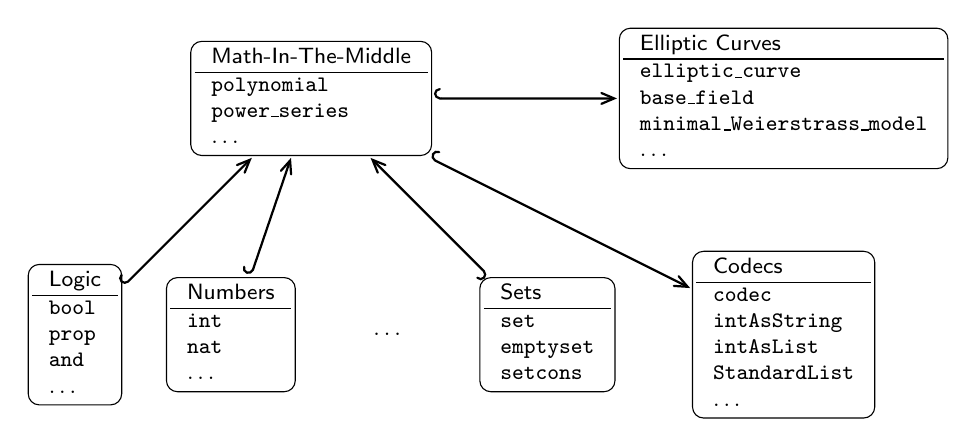
\begin{tikzpicture}[xscale=\myxscale,yscale=\myyscale]\myfontsize

  % Math-In-The-Middle and Components

  \node[thy] (mitm) at (1,1) {
    \begin{tabular}{l}
      \textsf{Math-In-The-Middle}\\\hline
      \texttt{polynomial}\\
      \texttt{power\_series}\\
      \dots
    \end{tabular}
  };

  \node[thy] (mitmlogic) at (0,-1) {
    \begin{tabular}{l}
      \textsf{Logic}\\\hline
      \texttt{bool}\\
      \texttt{prop}\\
      \texttt{and}\\
      \dots
    \end{tabular}
  };

  \node[thy] (mitmint) at (0.66,-1) {
    \begin{tabular}{l}
      \textsf{Numbers}\\\hline
      \texttt{int}\\
      \texttt{nat}\\
      \dots
    \end{tabular}
  };

  \node[draw,draw=white] (mitmdots) at (1.33,-1) {\dots};

  \node[thy] (mitmsets) at (2,-1) {
    \begin{tabular}{l}
      \textsf{Sets}\\\hline
      \texttt{set}\\
      \texttt{emptyset}\\
      \texttt{setcons}
    \end{tabular}
  };

  \draw[include] (mitmlogic) -- (mitm);
  \draw[include] (mitmint) -- (mitm);
  \draw[include] (mitmsets) -- (mitm);


  % Curves and Codecs

  \node[thy] (curve) at (3,1) {
    \begin{tabular}{l}
      \textsf{Elliptic Curves}\\\hline
      \texttt{elliptic\_curve}\\
      \texttt{base\_field}\\
      \texttt{minimal\_Weierstrass\_model}\\
      \dots
    \end{tabular}
  };

  \node[thy] (codecs) at (3,-1) {
    \begin{tabular}{l}
      \textsf{Codecs}\\\hline
      \codec\\
      \intAsString\\
      \intAsList\\
      \standardList\\
      \dots
    \end{tabular}
  };

  \draw[include] (mitm) -- (curve);
  \draw[include] (mitm) -- (codecs);
\end{tikzpicture}
\end{document}

%%% Local Variables:
%%% mode: latex
%%% TeX-master: t
%%% End:
           
  \caption[Theories involved in our architecture]{A Theory Graph of some of the theories (excluding their meta-theories)
    involved in \pn.  Symbols are listed underneath the theory name, and includes are represented as solid edges.  We omit the full
    declarations and some of the more fine-grained structure for simplicity.  }
  \label{fig:odk_theories}
\end{figure}


Most systems (including most systems involved in \pn) focus on the third level only.
The second level is usually left implicit, e.g.~because it is hard-coded in the implementation of the computation system.
Because the second level is hard-coded, there is then no need for the first level.
For system integration, it is important to make the second level explicit so that the semantics of the exchanged knowledge can be specified.
Thus, \MMT already anticipates much of the high-level concepts needed for the system-spanning \DKS-bases in \pn.

\paragraph{Theory Morphisms}
There are two kinds of theory morphisms: imports and views.  Imports are central for
building theories modularly by pulling together symbols introduced in other theories.
Practically, imports can be interpreted as copying symbol declarations while
instantiating, renaming, or otherwise modifying them.  The semantics of theories with
imports is defined categorially via colimits.

A view from theory $S$ to theory $T$ is a translation of $S$-objects to $T$-objects.
Contrary to imports, views are given after the involved theories have been defined.  Thus,
they have the character of theorems rather than definitions, and indeed views usually
induce proof obligations that must be discharged for a view to be accepted.  In the
presence of appropriate logical frameworks, \MMT guarantees a critical property: the
translation of objects preserves all properties of the type system and the logic.
\emph{In particular, all $S$-theorems are translated to $T$-theorems by views}.

Views are mainly used for the \emph{integration of knowledge} that comes from different
sources. Say system $A$ defines a group as an associative quasigroup with identity over an
operation $/$  (in a theory $G_A$), and system $B$ as a monoid with inverses for an
operation $\circ$ (in a theory $G_B$), then we can build a theory isomorphism (a pair of
mutually inverse views) that relates the two group theories $G_A$ and $G_B$ and allows to
transport all theorems between the two theories -- and consequently all algorithms between
the two systems $A$ and $B$. The modularity of the OMDoc/MMT system and an elaborate
calculus of theory morphisms make the establishment and management of views effective.

\paragraph{Implementation}
Theory graphs are implemented in the \MMT system~\cite{Rabe:MAGMS13,uniformal:on}.
At its core, this system allows for the declaration of theories along with symbols, imports and views, to build objects and translate them along views.

On top of this, the \MMT system provides a number of logical and knowledge management services.
The former includes computing the respective colimits, translating objects along morphisms, or type checking and proving objects relative to the respective meta-theory.
The latter include import/export of libraries, editing, browsing, and middleware for system integration.

%%% Local Variables:
%%% mode: latex
%%% TeX-master: "report"
%%% End:

%  LocalWords:  RabKoh textbf lst mmt-odk-int texttt non-prinable lstinputlisting emph pn
%  LocalWords:  mathescape odk_theories centering providecommand myxscale myyscale tikz
%  LocalWords:  myfontsize categorially colimits quasigroup circ isomoprhism
